\chapter{General Statistical Estimation and Inference}
\label{chap:est} 

Earlier, we often referred to certain estimators as being ``natural.''
For example, if we are estimating a population mean, an obvious choice
of estimator would be the sample mean.  But in many applications, it is
less clear what a ``natural'' estimate for a population quantity of
interest would be.  We will present general methods for estimation in
this section.

We will also discuss advanced methods of inference.

\section{General Methods of Parametric Estimation}
\label{genest}

Let's begin with a simple motivating example.

\subsection{Example:  Guessing the Number of Raffle Tickets Sold}
\label{raffle}

You've just bought a raffle ticket, and find that you have ticket number
68.  You check with a couple of friends, and find that their numbers are
46 and 79.  Let c be the total number of tickets.  How should we
estimate c, using our data 68, 46 and 79?

Let $X_1,X_2,...,X_n$ denote the ticket numbers we are aware of.  In the
above case, $n = 3$, with $X_1 = 68$ etc.  We will treat the $X_i$ as a
random sample from 1,2,...,c.  This assumption should be carefully
considered.  Recall that this means that $X_1,X_2,...,X_n$ are i.i.d.
with a (discrete) uniform distribution on 1,2....,c.  

If we know, say, that the three friends bought their tickets right after
they became available.  This might mean the $X_i$ are nearer to 1 than
to c, in which case the assumption of the uniform distribution may not
be very good.  Or, suppose we know that the three friends were standing
close to each other in line.  Then the independence assumption might be
dubious.  

And even if not, and even if the $X_i$ are considered a sample with the
uniformity assumption satisfied, it would technically be what is called
a {\it simple} random sample (Section \ref{randomsamples}), since the
``sampling'' is done without replacement; no two people get the same
ticket.

So, in practice one would need to consider how good our assumption is
that we have a random sample.  If $n << c$, the various probabilities
are virtually identical for sampling with and without replacement, so
that may not be an issue, so we would just worry about the uniformity.

But let's suppose that has been resolved, and then look at how we can
estimate c.

% It is reasonable to assume that each of the three of you is equally
% likely to get assigned any of the numbers 1,2,...,c.  In other words,
% the numbers we get, $X_i$, i = 1,2,3 are uniformly distributed on the
% set \{1,2,...,c\}.  We can also assume that they are independent; that's
% not exactly true, since we are sampling without replacement, but for
% large c---or better stated, for n/c small---it's close enough.  
 
\subsection{Method of Moments}
\label{mome}

One approach, a very intuitive one, is the Method of Momentsi (MM).  It
is less commonly used than the other method we'll cover, Maximum
Likelihood, but is much easier to explain.  Also, in recent years, MM
has become more popular in certain fields, such as random graph models
(Section \ref{randomgraph}).

\subsubsection{Example:  Lottery Model}

Let $X$ be distributed the same as the $X_i$, i.e.\ it is uniformly
distributed on 1,2,...,c.

Note first that 

\begin{equation}
\label{exinc}
E(X) = \frac{c+1}{2}
\end{equation}

Let's solve for c:

\begin{equation}
\label{cinex}
c = 2 EX - 1
\end{equation}

We know that we can use

\begin{equation}
\overline{X} = \frac{1}{n} \sum_{i=1}^{n} X_i
\end{equation}

to estimate EX, so by (\ref{cinex}), $2 \overline{X} - 1$ is an
intuitive estimate of c.  Thus we take our estimator for c to be

\begin{equation}
\label{cinexhat}
\widehat{c} = 2 \overline{X} - 1
\end{equation}

This estimator is called the Method of Moments estimator of c.

% \checkpoint

\subsubsection{General Method}

Say our sample is $X_1,...,X_n;a, and$ we have $k$ parameters to
estimate, $\theta_1,...,\theta_k$.  Our goal is to come up with
estimators $\widehat{\theta_1},...,\widehat{\theta_k}$.  

Here is the procedure:

\begin{itemize}

\item For each $i = 1,...,k$, write $E(X^k)$ as a function of the
$\theta_j$,

\begin{equation}
\label{moment}
E(X^i) = g_i(\theta_1,...,\theta_k)
\end{equation}

\item On the left side of (\ref{moment}), replace $E(X^i)$ by the
corresponding sample moment

\begin{equation}
\label{sammoment}
\frac{1}{n} \sum_{r=1}^n X_r^i
\end{equation}

\item On the right side of (\ref{moment}), replace each $\theta_s$ by
$\widehat{\theta_s}$.

\item Solve for the $\widehat{\theta_s}$

\end{itemize}

In the raffle example, we had k = 1, $\theta_1 = c$,
$g_1(c) = (c+1)/2$ and so on.  

\subsection{Method of Maximum Likelihood}
\label{mle}

Another method, much more commonly used, is called the {\bf Method of
Maximum Likelihood}.  

\subsubsection{Example:  Raffle Model}

In our example above, it means asking the
question, ``What value of c would have made our data---68, 46, 79---most
likely to happen?''  Well, let's find what is called the {\bf
likelihood}, i.e.\ the probability of our particular data values occurring:

\begin{equation}
\label{1stlike}
L = P(X_1 = 68, X_2 = 46, X_3 = 79) = 
\begin{cases} 
(\frac{1}{c})^3, & \text{if $c \geq 79$} \\ 
0, & \text{otherwise} \\ 
\end{cases} 
\end{equation}

Now keep in mind that c is a fixed, though unknown constant.  It is not
a random variable.  What we are doing here is just asking ``What if''
questions, e.g. ``If c were 85, how likely would our data be?  What
about c = 91?''

Well then, what value of c maximizes (\ref{1stlike})?  Clearly, it is c
= 79.  Any smaller value of c gives us a likelihood of 0.  And for c
larger than 79, the larger c is, the smaller (\ref{1stlike}) is.  So,
our maximum likelihood estimator (MLE) is 79.  In general, if our sample
size in this problem were n, our MLE for c would be

\begin{equation}
\check{c} = \max_i X_i
\end{equation}

Note that in our earlier discussion of whether our data can be treated
as a random sample, we raised the issue of the independence assumption.
Note that this assumption in fact {\it was} used for $\check{c}$, while
it was not for $\widehat{c}$.

\subsubsection{General Procedure}

Say again our random sample is $X_1,...,X_n$ and we have $k$ parameters to
estimate, $\theta_1,...,\theta_k$.  Our goal is to come up with
estimators $\widehat{\theta_1},...,\widehat{\theta_k}$.  

Denote the pmf or density of our $X_i$ as $f(t;\theta_1,...,\theta_k)$.
Then our estimators $\widehat{\theta_i}$ are the values that maximize
the likelihood

\begin{equation}
\Pi_{i=1}^n f(X_i; \theta_1,...,\theta_k)
\end{equation}

with respect to the $\theta_j$.  

For ``smooth'' problems, i.e.\ ones in which the likelihood is a
differentiable function of the parameters, aaximization involves taking
the derivatives with respect to the $\theta_j$, setting them to 0, then
solving for the $\theta_j$; the solutions are the
$\widehat{\theta_j}$.  

Since it is easier to take derivatives of sums than products, typically
one maximizes the log likelihood

\begin{equation}
\label{loglike}
\sum_{i=1}^n \ln[f(X_i; \theta_1,...,\theta_k)]
\end{equation}

\subsection{Example:  Estimation of the Parameters of a Gamma Distribution}
\label{gammamle}

As another example, suppose we have a random sample $X_1,...,X_n$ from 
a gamma distribution.

\begin{equation}
\label{gamma}
f_X(t) = \frac{1}{\Gamma(c)} \lambda^c t^{c-1} e^{-\lambda t}, ~ t > 0
\end{equation}

for some unknown $c$ and $\lambda$.  How do we estimate $c$ and
$\lambda$ from the $X_i$?

\subsubsection{Method of Moments}

Let's try the Method of Moments, as follows.  We have two population
parameters to estimate, c and $\lambda$, so we need to involve two
moments of X.  That could be EX and $E(X^2)$, but here it would more
conveniently be EX and Var(X).  We know from our previous unit on
continuous random variables, Chapter \ref{chap:contin}, that 

\begin{equation}
EX = \frac{c}{\lambda}
\end{equation}

\begin{equation}
Var(X) = \frac{c}{\lambda^2}
\end{equation}

In our earlier notation, this would be r = 2, $\theta_1 = c$ , $\theta_2
= \lambda$ and $g_1(c,\lambda) = c/\lambda$ and $g_2(c,\lambda) =
c/\lambda^2$.

Switching to sample analogs and estimates, we have

\begin{equation}
\frac{\widehat{c}}{\widehat{\lambda}} = \overline{X}
\end{equation}

\begin{equation}
\frac{\widehat{c}}{\widehat{\lambda} ^ 2} = s^2
\end{equation}

Dividing the two quantities yields

\begin{equation}
\widehat{\lambda} = \frac{\overline{X}}{s^2}
\end{equation}

which then gives

\begin{equation}
\widehat{c} = \frac{\overline{X}^2}{s^2}
\end{equation}

\subsubsection{MLEs}

What about the MLEs of c and $\lambda$?  Remember, the $X_i$ are
continuous random variables, so the likelihood function, i.e. the analog
of (\ref{1stlike}), is the product of the density values:

\begin{eqnarray}
L &=& 
   \Pi_{i=1}^n 
   \left [
   \frac{1}{\Gamma(c)} \lambda^c {X_i}^{c-1} e^{-\lambda {X_i}} 
   \right ] \\ 
&=& [\lambda^c/\Gamma(c)]^n 
\left ( \Pi_{i=1}^n X_i \right )^{c-1}
e^{-\lambda \sum_{i=1}^n X_i}
\end{eqnarray}

In general, it is usually easier to maximize the log likelihood
(and maximizing this is the same as maximizing the original likelihood):

\begin{equation}
\label{2ndlike}
l = (c-1) \sum_{i=1}^n \ln(X_i) - \lambda \sum_{i=1}^n X_i 
+ nc \ln(\lambda) - n \ln(\Gamma(c))
\end{equation}

One then takes the partial derivatives of (\ref{2ndlike}) with respect
to c and $\lambda$, and sets the derivatives to zero.  The solution
values, $\check{c}$ and $\check{\lambda}$, are then the MLEs of c and
$\lambda$.  Unfortunately, in this case, these equations do not have
closed-form solutions.  So the equations must be solved numerically.
(In fact, numerical methods are needed even more in this case, because
finding the derivative of $\Gamma(c)$ is not easy.)  

\subsection{R's mle() Function}

R provides a function, {\bf mle()}, for finding MLEs in mathematically
intractable situations such as the one in the last section.  

Note:  The function is in the {\bf stats4} library, so run

\begin{lstlisting}
> library(stats4)
\end{lstlisting}

first.

Here's an example in that context.  We'll simulate some data from a
gamma distribution with given parameter values, then pretend we don't
know those, and find the MLEs from the data:

\begin{Verbatim}[fontsize=\relsize{-2}]
> n <- 1000
> x <- rgamma(n,shape=2,rate=1)  # Erlang, r = 2, lambda is 1

# function to compute negative log likelihood
ll <- function(c,lambda) {
   loglik <- (c-1) * sum(log(x)) - sum(x)*lambda + n*c*log(lambda) -
      n*log(gamma(c))
   -loglik
}

summary(mle(minuslogl=ll,start=list(c=1.5,lambda=2)))
Maximum likelihood estimation

Call:
mle(minuslogl = ll, start = list(c = 1, lambda = 1))

Coefficients:
       Estimate Std. Error
c      2.147605 0.08958823
lambda 1.095344 0.05144393

-2 log L: 3072.181 
\end{Verbatim}

How did this work?  The main task we have is to write a function that
calculates the negative log likelihood, with that function's arguments
will be the parameters to be estimated.  We defined our function and
named it {\bf ll()}.\footnote{Note that in R, {\bf log()} calculates the
natural logarithm by default.}

Fortunately for us, {\bf mle()} calculates the derivatives numerically
too, so we didn't need to specify them in the log likelihood function.
(Needless to say, this function thus cannot be used in a problem in
which derivatives cannot be used, such as the lottery example above.)

We also need to supply {\bf mle()} with initial guesses for the
parameters.  That's done in the {\bf start} argument.  I more or less
arbitrarily chose these values.  You may have to experiment,
though, as some sets of initial values may not result in convergence.

The standard errors of the estimated parameters are also printed out,
enabling the formation of confidence intervals and significance tests.
(See Section \ref{stderrest} for the case of confidence intervals.)  In
fact, you can get the estimated covariance matrix for the vector of
estimated parameters.  In our case here:

\begin{Verbatim}[fontsize=\relsize{-2}]
> mleout <- mle(minuslogl=ll,start=list(c=1.5,lambda=2))
> solve(mleout@details$hessian)
                 c      lambda
c      0.008026052 0.004093526
lambda 0.004093526 0.002646478
\end{Verbatim}

By the way, there were also some warning messages, due to the fact that
during the iterative maximization process, some iterations generated
guesses for $\check{\lambda}$ were 0 or near it, causing problems with
{\bf log()}.

Maximizing the likelihood meant minimizing the negative log likelihood.
Why did the authors of R write it this way, and in fact report -2 times
the log likelihood?  The answer is that this is related to a
significance testing procedure, the {\it likelihood ratio test}, a
matter beyond the scope of this book.

Note that if you are using {\bf mle()} with a parametric family for
which R supplies a density function, it's quite convenient to simply use
that in our likelihood function code:

\begin{lstlisting}
> ll <- function(c,lambda) -sum(dgamma(x,shape=c,rate=lambda,log=TRUE))
> summary(mle(minuslogl=ll,start=list(c=1.5,lambda=2)))
Maximum likelihood estimation

Call:
mle(minuslogl = ll, start = list(c = 1.5, lambda = 2))

Coefficients:
       Estimate Std. Error
c      2.147605 0.08958823
lambda 1.095344 0.05144393

-2 log L: 3072.181 
\end{lstlisting}

R made things so convenient that we didn't even need to take the logs
ourselves.

\subsection{R's gmm() Function}

A function to do Method of Moments estimation is also available, in R's
{\bf gmm} package on CRAN.  The package actually does more, something
called Generalized Method of Moments, but we'll see how to use it in
elementary form here.

The work is done by the eponymous function {\bf gmm()}.  In our usage
here, the call form is

\begin{lstlisting}
gmm(data,momentftn{,start)}
\end{lstlisting}

where {\bf data} is our data in matrix or vector form, {\bf momentftn}
specifies the moments, and {\bf start} is our initial guess for the
iterative solution process.

The function {\bf momentftn()} specifies how to compute the differences
between the estimated values of the population moments (in terms of the
parameter estimates) and the corresponding sample powers. During the
computation, {\bf gmm()} will set the means of these differences to 0,
iterating until convergence.

\subsubsection{Example:  Bodyfat Data}

Our data set will be {\bf bodyfat}, which is included in the {\bf mfp}
package, with measurements on 252 men. The first column of this data
frame, {\bf brozek}, is the percentage of body fat, which when converted
to a proportion is in (0,1). That makes it a candidate for fitting a
beta distribution (Section \ref{betafamily}).

Here is our {\bf momentftn()}:

\begin{lstlisting}
g <- function(th,x) {
   t1 <- th[1]
   t2 <- th[2]
   t12 <- t1 + t2
   meanb <- t1 / t12
   m1 <- meanb - x
   m2 <- t1*t2 / (t12^2 * (t12+1)) - (x - meanb)^2
   f <- cbind(m1,m2)
   return(f)
}
\end{lstlisting}

Here the argument {\bf th} (“theta”) will be the MM estimates (at any
given iteration) of the population parameters, in this case of 
$\alpha$ and $\beta$.  

Now look at the line

\begin{lstlisting}
m1 <- meanb - x
\end{lstlisting}

The value {\bf meanb} is our estimate in the currently iteration of the
mean of the beta distribution, while {\bf x} is our data.  The {\bf
gmm()} function, in calling our {\bf g()}, will calculate the average of
{\bf m1} over all our data, and then in setting that average to 0, we
are equating our parametric estimate of the population mean to our
sample mean --- exactly what MM is supposed to do.

Let's try it:

\begin{lstlisting}
> library(mfp)
> data(bodyfat)
> gmm(g,x,c(alpha=0.1,beta=0.1))
Method
 twoStep 

Objective function value: 2.559645e-10 

 alpha beta 
 4.6714 19.9969 

Convergence code = 0 
> hist(bodyfat$brozek/100,xlim=c(0,1),
   probability=TRUE)
> curve(dbeta(x,4.67,20.00),add=TRUE)
\end{lstlisting} 

The result is seen in Figure \ref{betafit}.  At least visually, the
fit seems pretty good.

\begin{figure}
\centerline{
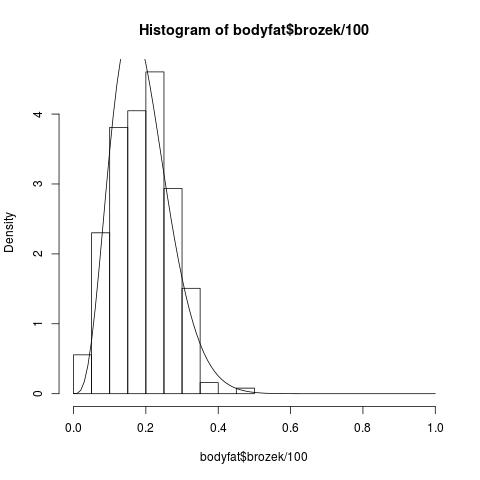
\includegraphics[width=5.0in]{Bodyfat.jpg}
}
\caption{Fitting a Beta Density}
\label{betafit}
\end{figure}



\subsection{More Examples}

Suppose $f_W(t) = ct^{c-1}$ for t in (0,1), with the density
being 0 elsewhere, for some unknown $c > 0$.  We have a random sample
$W_1,...,W_n$ from this density.  

Let's find the Method of Moments estimator.

\begin{equation}
EW = \int_{0}^{1} t ct^{c-1}~ dt = \frac{c}{c+1}
\end{equation}

So, set

\begin{equation}
\overline{W} = \frac{\widehat{c}}{\widehat{c}+1}
\end{equation}

yielding

\begin{equation}
\label{chatmom}
\widehat{c} = \frac{\overline{W}}{1-\overline{W}}
\end{equation}

What about the MLE?

\begin{equation}
L = \Pi_{i=1}^n c W_i^{c-1} 
\end{equation} 

so

\begin{equation}
l = n \ln{c} + (c-1) \sum_{i=1}^{n} \ln{W_i}
\end{equation}

Then set

\begin{equation}
0 = \frac{n}{\widehat{c}} + \sum_{i=1}^{n} \ln{W_i}
\end{equation}

and thus

\begin{equation}
\label{widehatc}
\widehat{c} = -\frac{1}{\frac{1}{n} \sum_{i=1}^{n} \ln{W_i}}
\end{equation}

% Note that we don't need the delta method to find a confidence interval
% here, as we can rewrite (\ref{chatmom}) as
% 
% \begin{equation}
% \widehat{c} = \frac{1}{\frac{1}{\overline{W}}-1}
% \end{equation}

As in Section \ref{mle}, not every MLE can be determined by taking
derivatives.  Consider a continuous analog of the example in that
section, with $f_W(t) = \frac{1}{c}$ on (0,c), 0 elsewhere, for some
$c > 0$. 

The likelihood is

\begin{equation}
\left ( \frac{1}{c} \right )^n
\end{equation}

as long as

\begin{equation}
c \geq \max_i W_i
\end{equation}

and is 0 otherwise.  So,

\begin{equation}
\label{unifmle}
\widehat{c} = \max_i W_i
\end{equation}

as before.

Now consider a different problem.  Suppose the random variable X is
equal to 1, 2 and 3, with probabilities c, c and 1-2c.  The value c is
thus a population parameter.  We have a random sample $X_1,...,X_n$ from
this population.  Let's find the Method of Moments Estimator of c, and
its bias.

First,

\begin{equation}
EX = c \cdot 1 + c \cdot 2 + (1-2c) \cdot 3 = 3 - 3c
\end{equation}

Thus 

\begin{equation}
c = (3-EX)/3
\end{equation}

and so set

\begin{equation}
\hat{c} = (3-\overline{X})/3
\end{equation}

Next,

\begin{eqnarray}
E \hat{c} &=& E[(3-\overline{X})/3) \\ 
&=& \frac{1}{3} \cdot (3 - E\overline{X}) \\
&=& \frac{1}{3} [ 3 - EX ] \\
&=& \frac{1}{3} [ 3 - (3-3c) ] \\
&=& c
\end{eqnarray}

On average, not too high and not too low; we say the {\it bias} is 0.

\subsection{Asymptotic Properties}

Most of the inference methods in this book use large-sample, i.e.\ {\it
asymptotic} techniques, based on the Central Limit Theorem.  Let's look
at the asymptotic properties of Method of Moments and Maximum Likelihood
estimators.

\subsubsection{Consistency}

We say that an estimator $\widehat{\nu}$ of some parameter $\nu$ is
{\bf consistent} if, with probability 1,

\begin{equation}
\lim_{{n} \rightarrow \infty} \widehat{\nu} = \nu
\end{equation}

where n is the sample size.  In other words, as the sample size grows,
the estimator eventually converges to the true population value.
Clearly, in most situations consistency is a minimal property we want
our estimators to have.

Of course here $\overline{X}$ is a consistent estimator of EX, and
(\ref{sammoment}) is a consistent estimator of $E(X^i)$.  So, as long as
the $g_i()$ in (\ref{sammoment}) are continous etc., we see that the
Method of Moments gives us consistent estimators.

Showing consistency for MLEs is a little more involved.  To start,
recall (\ref{loglike}).  Its derivative with respect to $\theta_j$ is

\begin{equation}
\label{llprime}
\sum_{i=1}^n 
\frac
{f'(X_i; \theta_1,...,\theta_k)}
{f(X_i; \theta_1,...,\theta_k)}
\end{equation}

For each value of $\theta = (\theta_1,...,\theta_k)'$, this will
converge to 

\begin{equation}
\label{llprimelim}
E \left (
\frac{f'(X;\theta)}
     {f(X;\theta)}
\right )
\end{equation}

Let $\eta$ denote the true population value of $\theta$, with
$\widehat{\theta}$ being the MLE.  The latter is the root of
(\ref{llprime}), 

\begin{equation}
0 = \sum_{i=1}^n 
\frac
{f'(X_i; \widehat{\theta})}
{f(X_i; \widehat{\theta})}
\end{equation}

Moreover, in for instance the continuous case (we'll be implicitly
assuming some mathematical conditions here, e.g.\ that roots are uniqe),

\begin{eqnarray}
E \left (
\frac{f'(X;\eta)}
     {f(X;\eta)}
     \right ) &=&
\int_{-\infty}^{\infty} f'(t;\eta) ~ dt \\
&=& \frac{d}{dt}\int_{-\infty}^{\infty} f(t;\eta) ~ dt \\
&=& \frac{d}{dt} 1 \\
&=& 0
\end{eqnarray}

Due to the uniqeness of the roots, we see that $\widehat{\\theta}$, 
the root of (\ref{llprime}) must converge to $\eta$, the root of
(\ref{llprimelim}).

\subsubsection{Approximate Confidence Intervals}

Usually we are not satisfied with simply forming estimates (called {\bf
point estimates}).  We also want some indication of how accurate these
estimates are, in the form of confidence intervals ({\bf interval
estimates}).

In many special cases, finding confidence intervals can be done easily
on an {\it ad hoc} basis.  Look, for instance, at the Method of Moments
Estimator in Section \ref{mome}.  Our estimator (\ref{cinexhat}) is a
linear function of $\overline{X}$, so we easily obtain a confidence
interval for $c$ from one for $EX$.

Another example is (\ref{widehatc}).  Taking the limit as $n \rightarrow
\infty$ the equation shows us (and we could verify) that 

\begin{equation}
\label{cintermsofw}
c = \frac{1}{E[\ln{W}]}
\end{equation}

Defining $X_i = \ln{W_i}$ and $\overline{X} = (X_1+...+X_n)/$, we can
obtain a confidence interval for $EX$ in the usual way.  We then see
from (\ref{cintermsofw}) that we can form a confidence interval for $c$
by simply taking the reciprocal of each endpoint of the interval, and
swapping the left and right endpoints.

What about in general?  For the Method of Moments case, our estimators
are functions of the sample moments, and since the latter are formed
from sums and thus are asymptotically normal, the delta method (Section
\ref{delta}) can be used to show that our estimators are asymptotically
normal and to obtain asymptotic variances for them.

There is a well-developed asymptotic theory for MLEs, which under
certain conditions shows asymptotic normality with a certain asymptotic
variance, thus enabling confidence intervals.  The theory also
establishes that MLEs are in a certain sense optimal among all
estimators.  We will not pursue this here, but will note that {\bf mle()}
does give standard errors for the estimates, thus enabling the
formation of confidence intervals.

\section{Bias and Variance}
\label{bv}

The notions of {\bf bias} and {\bf variance} play central roles in the
evaluation of goodness of estimators.

\subsection{Bias}

{\it This bowl of porridge is not too big, not too small, but just
right}---from the children's story, {\it Goldilocks} (paraphrased)

\begin{definition}
Suppose $\hat{\theta}$ is an estimator of $\theta$.
Then the {\bf bias} of $\hat{\theta}$ is 

\begin{equation}
\textrm{bias} = E(\hat{\theta}) - \theta
\end{equation}

If the bias is 0, we say that the estimator is {\bf unbiased}.
\end{definition}

So, if $\hat{\theta}$ is an unbiased estimator of $\theta$, then its
average value over all possible samples is not too high, not too low,
but just right.

At first that would seem to be a ``must have'' property for any
estimator.  But it's very important to note that, in spite of the
pejorative-sounding name, bias is not an inherently bad property for an
estimator to have.  Indeed, most good estimators are at least slightly
biased.\footnote{Typically, though, the amount of bias will go to 0 as
the sample size goes to infinity.  That is the case for most consistent
estimators (Sec. \ref{mome}, though technically it is not implied by
consistency; if a sequence of random variables converges to a limit,
their expected values do not necessarily converge to that limit, or
converge at all).} We'll explore this in the next section.

\subsection{Why Divide by n-1 in $s^2$?}  
\label{whynot}

It should be noted that it is customary in (\ref{s2}) to divide by n-1
instead of n, for reasons that are largely historical.  Here's the
issue:

If we divide by n, as we have been doing, then it turns out that
$s^2$ is biased.

\begin{equation}
\label{s2biased}
E(s^2) = \frac{n-1}{n} \cdot \sigma^2
\end{equation}

Think about this in the Davis people example, once again in the notebook
context.  Remember, here n is 1000, and each line of the notebook
represents our taking a different random sample of 1000 people.  Within
each line, there will be entries for  $W_1$ through $W_{1000}$, the
weights of our 1000 people, and for $\overline{W}$ and $s$.  For convenience,
let's suppose we record that last column as $s^2$ instead of $s$.

Now, say we want to estimate the population variance $\sigma^2$.  As
discussed earlier, the natural estimator for it would be the sample
variance, $s^2$.  What (\ref{s2biased}) says is that after looking at an
infinite number of lines in the notebook, the average value of $s^2$
would be just...a...little...bit...too...small.  All the $s^2$ values
would average out to $0.999 \sigma^2$, rather than to $\sigma^2$.  We
might say that $s^2$ has a little bit more tendency to underestimate 
$\sigma^2$ than to overestimate it.

So, (\ref{s2biased}) implies that $s^2$ is a biased estimator of the
population variance $\sigma^2$, with the amount of bias being

\begin{equation}
\frac{n-1}{n} \cdot \sigma^2 - \sigma^2 = -\frac{1}{n} \cdot \sigma^2
\end{equation}

Let's prove (\ref{s2biased}).  As before, let $W_1,...,W_n$ be a random
sample from some population.  So, $EW_i = \mu$ and $Var(W_i) =
\sigma^2$, where again $\mu$ and $\sigma^2$ are the population mean and
variance.

It will be more convenient to work with $ns^2$ than $s^2$, since it will
avoid a lot of dividing by n.  So, write

\begin{eqnarray}
ns^2 &=& \sum_{i=1}^n (W_i - \overline{W})^2 ~~~~ \textrm{(def.)} \\
&=& \sum_{i=1}^n 
\left [
(W_i - \mu) + (\mu - \overline{W})
\right ]^2 ~~~~ \textrm{(alg.)} \\
&=& 
\sum_{i=1}^n (W_i - \mu)^2 +
2 (\mu - \overline{W}) \sum_{i=1}^n (W_i - \mu) +
n (\mu - \overline{W})^2 ~~~~ \textrm{(alg.)}
\end{eqnarray}

But that middle sum is 

\begin{equation}
\sum_{i=1}^n (W_i - \mu) =
\sum_{i=1}^n W_i - n \mu =
n \overline{W} - n \mu
\end{equation}

So,

\begin{equation}
\label{intermed}
ns^2 = \sum_{i=1}^n (W_i - \mu)^2  - n (\overline{W} - \mu)^2 
\end{equation}

Now let's take the expected value of (\ref{intermed}).  First,

\begin{eqnarray}
E \left (
\sum_{i=1}^n (W_i - \mu)^2
\right )
&=& \sum_{i=1}^n E[(W_i - \mu)^2] ~~~~ \textrm{(E is lin.)} \\ 
&=& \sum_{i=1}^n E[(W_i - EW_i)^2] ~~~~ (W_i \textrm{ distr. as pop.}) \\ 
&=& \sum_{i=1}^n Var(W_i) ~~~~ \textrm{(def. of Var())} \\ 
&=& \sum_{i=1}^n \sigma^2 ~~~~ (W_i \textrm{ distr. as pop.}) \\ 
&=& n \sigma^2
\end{eqnarray}

Also,

\begin{eqnarray}
E[(\overline{W} - \mu)^2] &=& 
   E[(\overline{W} - E\overline{W})^2] ~~~~ ((\ref{barmean})) \\ 
&=& Var(\overline{W}) ~~~~ \textrm{ (def. of Var())} \\
&=& \frac{\sigma^2}{n} ~~~~ (\ref{oneovernpopvar})
\end{eqnarray}

Applying these last two findings to (\ref{intermed}), we get
(\ref{s2biased}).

% Write the first term as
% 
% \begin{eqnarray}
% E \left ( \frac{1}{n}\sum_{i=1}^n W_i^2 \right ) &=&  
% \frac{1}{n}E \sum_{i=1}^n W_i^2 ~~ \textrm{  (constants factor out of E())} \\
% &=& \frac{1}{n} \cdot n E(W^2) ~~ \textrm{  (each $W_i$ has distr. of W)} \\
% &=& E(W^2) \\
% &=& Var(W) + (EW)^2 \\
% &=& \sigma^2 + \mu^2
% \end{eqnarray}
% 
% Continuing to work from (\ref{alts2}) and using (\ref{oneovernpopvar}), write
% 
% \begin{equation}
% E[\overline{W}^2] = Var(\overline{W}) + [E(\overline{W})]^2 = \frac{1}{n} \sigma^2 +
% \mu^2
% \end{equation}
% 
% Now using all this in (\ref{alts2}), we get
% 
\begin{equation}
E(s^2) = \frac{n-1}{n} \sigma^2
\end{equation}

% \checkpoint

The earlier developers of statistics were bothered by this bias, so they
introduced a ``fudge factor'' by dividing by n-1 instead of n in
(\ref{s2}).  We will call that $\tilde{s}^2$:

\begin{equation}
\label{tildes2}
\tilde{s}^2 = 
\frac{1}{n-1} \sum_{i=1}^{n} (W_i-\overline{W})^2 
\end{equation}

This is the ``classical'' definition of sample variance, in which we
divide by n-1 instead of n.  

The R functions {\bf var()} and {\bf sd()} calculate the versions of
$s^2$ and $s$, respectively, that have a divisor of n-1.  In other
words, {\bf var()} calculates (\ref{tildes2}), and {\bf sd()} computes
its square root.

\subsubsection{But in This Book, We Divide by n, not n-1 Anyway}
\label{wearedifferent}

But we will use n.  After all, when n is large---which is
what we are assuming by using the Central Limit Theorem in most of the
inference machinery here---it doesn't make any appreciable difference.
Clearly it is not important in our Davis example, or our bus simulation
example.

Moreover, speaking generally now rather than necessarily for the case of
$s^2$ there is no particular reason to insist that an estimator be
unbiased anyway.  An alternative estimator may have a little bias but
much smaller variance, and thus might be preferable.  

And anyway, even though the classical version of $s^2$, i.e.
$\tilde{s}^2$, is an unbiased estimator for $\sigma^2$, $\tilde{s}$ is
not an unbiased estimator for $\sigma$, the population standard
deviation (see below).  Since we typically have use for $\tilde{s}$
rather than for $\tilde{s}^2$---in (\ref{meanci}), for example---you can
see that unbiasedness is not such an important property after all.

Let's show that $\tilde{s}$ is biased.  Recalling the shortcut
formula $Var(U) = E(U^2) - (EU)^2$, we have

\begin{eqnarray}
0 &<& Var(\tilde{s}) \label{sbias1} \\ 
&=& E[\tilde{s}^2] - [E\tilde{s}]^2    \\
&=& \sigma^2 - [E\tilde{s}]^2 \label{sbias2}
\end{eqnarray}

since $\tilde{s}^2$ is an unbiased estimator of $\sigma^2$.  So,

\begin{equation}
E\tilde{s} < \sigma
\end{equation}

and $\tilde{s}$ is biased downward.\footnote{The reader may wonder why
we have strict inequality in (\ref{sbias1}).   But although it tis rue
that Var(U) can be 0, you'll recall that that occurs only when
U is constant.  Here it would mean that $\tilde{s}$ is constant.  This
in turn would mean that all the $W_i$ in (\ref{tildes2}) are identical,
with probability 1.0---which would mean the population random variable W
is constant, e.g. everyone in Davis has the same weight.  So, other that
in that absurd situation, the inequality in (\ref{sbias1}) will indeed
be strict.}

So, $\tilde{s}$, the standard estimator of $\sigma$, is indeed biased, as
are many other standard estimators of various quantities.  It would be
futile to insist on unbiasedness as a criterion of the goodness of an
estimator.

\subsection{Example of Bias Calculation:  Max from U(0,c)}

Let's find the bias of the estimator (\ref{unifmle}).

The bias is $E\widehat{c} - c$.  To get $E\widehat{c}$ we need the
density of that estimator, which we get as follows:

\begin{eqnarray}
P(\widehat{c} \leq t) &=& P(\textrm{all} ~ W_i \leq t)  ~~ (\textrm{definition})\\
&=& \left ( \frac{t}{c} \right )^n ~~ (\textrm{density of } W_i)
\end{eqnarray}

So,

\begin{equation}
f_{\widehat{c}}(t) = \frac{n}{c^n}  t^{n-1}
\end{equation}

Integrating against t, we find that

\begin{equation}
\label{notbad}
E\widehat{c} = \frac{n}{n+1} ~ c
\end{equation}

So the bias is c/(n+1), not bad at all.

\subsection{Example of Bias Calculation:  Gamma Family}

Let us find via simulation, the bias of the Method of Moments Estimator
of the parameter $\lambda$ for the family of gamma distributions.
(The estimator was derived in Section \ref{gammamle}.)

\begin{lstlisting}
lambbias <- function(r,lamb,n,nreps) {
   lambhat <- vector(length=nreps)
   unfudge <- (n-1) / n
   for (i in 1:nreps) {
      x <- rgamma(n,shape=r,rate=lamb)
      xbar <- mean(x)
      s2 <- var(x) * unfudge
      lambhat[i] <- xbar / s2
   }
   mean(lambhat) - lamb
}
\end{lstlisting}

\subsection{Tradeoff Between Variance and Bias}
\label{msesection}

Consider a general estimator Q of some population value b.  Then a
common measure of the quality (of course there are many others) of the
estimator Q is the {\bf mean squared error} (MSE),

\begin{equation}
\label{mse}
E[(Q-b)^2]
\end{equation}

Of course, the smaller the MSE, the better.

One can break (\ref{mse}) down into variance and (squared) bias
components, as follows:\footnote{In reading the following derivation,
keep in mind that EQ and b are constants.}

\begin{eqnarray}
MSE(Q) &=& E[(Q-b)^2] \textrm{  (definition)} \\
&=& E[\{(Q-EQ) + (EQ - b)\}^2] \textrm{  (algebra)} \\
&=& E[(Q-EQ)^2] + 2 E \left [ (Q-EQ) (EQ-b) \right ] + E[ (EQ - b)^2 ]
\textrm{  (E props.)} \\
&=& E[(Q-EQ)^2] + E[ (EQ - b)^2 ] \textrm{  (factor out constant EQ-b)} \\
&=&  Var(Q) + (EQ - b)^2 
\textrm{  (def. of Var(), fact that EQ-b is const.)} 
\label{mseformula}\\
&=& \textrm{variance + squared bias} 
\label{vb2}
\end{eqnarray}

In other words, in discussing the accuracy of an estimator---especially
in comparing two or more candidates to use for our estimator---the
average squared error has two main components, one for variance and one
for bias.  In building a model, these two components are often at odds
with each other; we may be able to find an estimator with smaller bias
but more variance, or vice versa.

We also see from (\ref{vb2}) that a little bias in an estimator
may be quite tolerable, as long as the variance is low.  This is good,
because as mentioned earlier, most estimators are in fact biased.

These point will become central in Chapters \ref{chap:mod} and
\ref{chap:linreg}.

% \checkpoint

% \section{More on the Issue of Independence/Nonindependence of Samples}
% 
% In Section \ref{indepsams}, we derived confidence intervals for the
% difference between two population means (or proportions).  The
% derivation depended crucially on the fact that the two sample means,
% $\overline{X}$ and $\overline{Y}$, were independent.  This in turn
% stemmed from the fact that the corresponding sample data sets were
% separate.  
% 
% On the other hand, in Section \ref{depsams}, we had an example in which
% the two sample means, $\overline{X}$ and $\overline{Y}$, were not
% independent, as they came from the same set of kids.  The confidence
% intervals derived in Section \ref{indepsams} were thus invalid, and new
% ones were derived, based on differences.
% 
% Note that in both cases, the observations {\it within} a sample were
% also independent.  In the example of children's heights in Section
% \ref{depsams}, for instance, the fact that Mary was chosen as the first
% child in the sample had no effect on whether Jane was chosen as the
% second one.  This was important for the derivations too, as they used
% (\ref{oneovernpopvar}), which assumed independence.
% 
% In this section, we will explore these points further, with our aim
% being to state the concepts in precise random variable terms.  
% 
% As our concrete example, consider an election survey, in a small city.
% Say there are equal numbers of men and women in the city, 5000 each.  We
% wish to estimate the population proportion of people who plan to vote
% for candidate A.  We take a random sample of size n from the population,
% Define the following:
% 
% \begin{itemize}
% 
% \item Let V denote the indicator variable for the event that the person
% plans to vote for A.  
% 
% \item We might be interested in differences between men and women in A's
% support, so let G be 1 for male, 2 for female.  
% 
% \item Let $p$ denote the population proportion of people who plan to vote
% for A.
% 
% \item Let $p_1$ and $p_2$ denote the population proportions planning to
% vote for A, among men and women respectively.  Note that
% 
% \begin{equation}
% \label{pp1p2}
% p = 0.5 p_1 + 0.5 p_2
% \end{equation}
% 
% \item Denote our data by $(V_1,G_1),...,(V_n,G_n)$, recording both the
% planned vote and gender for each person in the sample.
% 
% \item For convenience, relabel the data by gender, with
% $M_1,...,M_{N_1}$ and $F_1,...,F_{N_2}$ denoting the planned votes of
% the men and women.
% 
% \end{itemize}
% 
% Clearly, the male data and female data are independent.  The fact that
% Jack is chosen in the male sample has no impact on whether Jill is
% chosen in the female one.
% 
% But what about data {\it within} a gender group?  For example, are $M_1$
% and $M_2$, the planned votes of the first two men in our male sample,
% independent?  Or are they correlated, since these two people have the
% same gender?
% 
% The answer is that $M_1$ and $M_2$ are indeed independent.  The first
% man could be any of the 5000 men in the city, with probability 1/5000
% each, and the same is true of the second man.  Moreover, the choice of
% the first man has no effect at all on the choice of the second one.
% (Remember, in random samples we sample {\it with} replacement.)
% 
% Our estimate of $p$ is our usual sample proportion,
% 
% \begin{equation}
% \widehat{p} = \frac{V_1+...+V_n}{n}
% \end{equation}
% 
% Then we can use (\ref{propci}) to find a confidence interval for $p$.
% But again, the reader might question this, saying something like, ``What
% if $G_1$ and $G_2$ are both 1, i.e. the first two people in our sample
% are both men?  Won't $V_1$ and $V_2$ then be correlated?''  The answer
% is no, because the reader would be referring to the conditional
% distribution of V given G, whereas our use of (\ref{propci}) does not
% involve gender, i.e. it concerns the unconditional distribution of V.
% 
% This point is subtle, and is difficult for the beginning modeler to
% grasp.  It is related to issues in our first discussions of probability
% in Chapter \ref{probcalc}.  In the ALOHA model there, for instance,
% beginning students who are asked to find $P(X_2 = 1)$ often object,
% ``Well, it depends on what $X_1$ is.''  That is incorrect thinking,
% because they are confusing $P(X_2 = 1)$ with $P(X_2 = 1 | X_1 = i)$.
% That confusion is resolved by thinking in ``notebook'' terms, with
% $P(X_2 = 1)$ meaning the long-run proportion of notebook lines in which
% $X_2 = 1$, \textit{regardless} of the value of $X_1$.  In our case
% here, the reader must avoid confusing $P(V = 1)$ (which is $p$) with
% $P(V = 1 | G = i)$ (which is $p_i$).
% 
% Continuing this point a bit more, note that our $\widehat{p}$ above {\it
% is} an unbiased estimate of $p$:
% 
% \begin{eqnarray}
% \label{phatunb}
% E \widehat{p} &=& E(V_1) ~~~~ ((\ref{barmean})) \\ 
% &=& P(V_1 = 1) ~~~~ ((\ref{eofxeqp})) \\
% &=& P(G_1 = 1) P(V_1 = 1 | G_1 = 1)
% + P(G_1 = 2) P(V_1 = 1 | G_1 = 2) ~~~~ (\textrm{Chapter } \ref{probcalc}) \\
% &=& 0.5 p_1 + 0.5 p_2 \\
% &=& p ~~~~ ((\ref{pp1p2})) 
% \end{eqnarray}
% 
% Due to the independence of the male and female samples, we can use
% (\ref{2indepsamp}) to find a confidence interval for $p_1 - p_2$, so
% that we can compare male and female support of A.  Note by the way that
% $\overline{M}$ will be an unbiased estimate of $p_1$, with a similar
% statement holding for the women.
% 
% Now, contrast all that with a different kind of sampling, as follows.
% We choose a gender group at random, and then {\it sample n people from
% \underline{that} gender group}.  Let R denote the group chosen, so that
% $G_i = R$ for all i.  So, what about the answers to the above questions
% in this new setting?
% 
% Conditionally on R, the $V_i$ are again independent, using the same
% argument as we used to show that $M_1$ and $M_2$ were independent above.
% And (\ref{phatunb}) still works, so our $\widehat{p}$ is still unbiased.
% 
% However:  The $V_i$ are no longer unconditionally independent:
% 
% \begin{equation}
% P(V_1 = 1 \textrm{ and } V_2 = 1) = 0.5 p_1^2 + 0.5 p_2^2
% \end{equation}
% 
% (the reader should fill in the details, with a conditioning
% argument like that in (\ref{phatunb})), while
% 
% \begin{equation}
% P(V_1 = 1) \cdot P(V_2 = 1) = p^2 = (0.5 p_1 + 0.5 p_2)^2
% \end{equation}
% 
% So, 
% 
% \begin{equation}
% P(V_1 = 1 \textrm{ and } V_2 = 1) \neq
% P(V_1 = 1) \cdot P(V_2 = 1) 
% \end{equation}
% 
% and thus $V_1$ and $V_2$ are not unconditionally independent.
% 
% This setting is very common.  We might, for instance, choose k trees
% at random, and then collect data on r leaves in each tree.

\section{Simultaneous Inference Methods} 
\label{simultaninfer} 

{\it Events of small probability happen all the time, because there are
so many of them}---Jim Sutton, old Cal Poly economics professor

Suppose in our study of heights, weights and so on of people in Davis,
we are interested in estimating a number of different quantities, with
our forming a confidence interval for each one.  Though our confidence
level for each one of them will be 95\%, our {\it overall} confidence
level will be less than that.  In other words, we cannot say we are 95\%
confident that all the intervals contain their respective population
values.

In some cases we may wish to construct confidence intervals in such a
way that we can say we are 95\% confident that all the intervals are
correct.  This branch of statistics is known as {\bf simultaneous
inference} or {\bf multiple inference}.  

(The same issues apply to significance testing, but we will focus on
confidence intervals here.)

In this age of Big Data, simultaneous inference is a major issue.  We
may have hundreds of variables, so the chances of getting spurious
results are quite high.

Usually this kind of methodology is used in the comparison of several
{\bf treatments}.  This term originated in the life sciences, e.g.
comparing the effectiveness of several different medications for
controlling hypertension, it can be applied in any context.  For
instance, we might be interested in comparing how well programmers do in
several different programming languages, say Python, Ruby and Perl.
We'd form three groups of programmers, one for each language, with say
20 programmers per group.  Then we would have them write code for a
given application.  Our measurement could be the length of time T that
it takes for them to develop the program to the point at which it runs
correctly on a suite of test cases.  

Let $T_{ij}$ be the value of T for the j$^{th}$ programmer in the
i$^{th}$ group, i = 1,2,3, j = 1,2,...,20.  We would then wish to
compare the three ``treatments,'' i.e. programming languages, by
estimating $\mu_i = ET_{i1}$, i = 1,2,3.  Our estimators would be $U_i =
\sum_{j=1}^{20} T_{ij}/20$, i = 1,2,3.  Since we are comparing the three
population means, we may not be satisfied with simply forming ordinary
95\% confidence intervals for each mean.  We may wish to form confidence
intervals which {\it jointly} have confidence level 95\%.\footnote{The
word {\it may} is important here.  It really is a matter of philosophy
as to whether one uses simultaneous inference procedures.}

Note very, very carefully what this means.  As usual, think of our
notebook idea.  Each line of the notebook would contain the 60
observations; different lines would involve different sets of 60 people.
So, there would be 60 columns for the raw data, three columns for the
$U_i$.  We would also have six more columns for the confidence intervals
(lower and upper bounds) for the $\mu_i$.  Finally, imagine three more
columns, one for each confidence interval, with the entry for each being
either Right or Wrong.  A confidence interval is labeled Right if it
really does contain its target population value, and otherwise is
labeled Wrong.

Now, if we construct individual 95\% confidence intervals, that means
that in a given Right/Wrong column, in the long run 95\% of the entries
will say Right.  But for simultaneous intervals, we hope that within a
line we see \underline{three} Rights, and 95\% of all lines will have
that property.

In our context here, if we set up our three intervals to have individual
confidence levels of 95\%, their simultaneous level will be $0.95^3 =
0.86$, since the three confidence intervals are independent.
Conversely, if we want a simultaneous level of 0.95, we could take each
one at a 98.3\% level, since $0.95^{\frac{1}{3}} \approx 0.983$.

However, in general the intervals we wish to form will not be
independent, so the above ``cube root method'' would not work.  Here we
will give a short introduction to more general procedures.

Note that ``nothing in life is free.''  If we want simultaneous
confidence intervals, they will be wider.

Another reason to form simultaneous confidence intervals is that it
gives you  ``license to browse,'' i.e. to rummage through the data
looking for interesting nuggets.

\subsection{The Bonferonni Method}

One simple approach is {\bf Bonferonni's Inequality}:

\begin{lemma}
Suppose $A_1,...,A_g$ are events.  Then

\begin{equation}
\label{bonf}
P(A_1 {\rm ~or~...~or} A_g) \leq \sum_{i=1}^{g} P(A_i)
\end{equation}

\end{lemma}

You can easily see this for g = 2: 

\begin{equation}
P(A_1 \textrm{ or } A_2) = P(A_1) + P(A_2) - P(A_1 \textrm{ and } A_2)
\leq  P(A_1) + P(A_2)
\end{equation}

One can then prove the general case by mathematical induction.

Now to apply this to forming simultaneous confidence intervals, take
$A_i$ to be the event that the $i^{th}$ confidence interval is
incorrect, i.e. fails to include the population quantity being
estimated.  Then (\ref{bonf}) says that if, say, we form two confidence
intervals, each having individual confidence level (100-5/2)\%, i.e.
97.5\%, then the overall collective confidence level for those two
intervals is at least 95\%.  Here's why:
Let $A_1$ be the event that the first interval is wrong, and $A_2$ is
the corresponding event for the second interval.  Then

% \checkpoint
\begin{eqnarray}
\textrm{overall conf. level} &=& P(\textrm{not } A_1 \textrm{ and not } A_2) \\ 
&=& 1 - P(A_1 \textrm{ or } A_2) \\
&\geq&  1 - P(A_1) - P(A_2) \\
&=& 1 - 0.025 - 0.025 \\
&=& 0.95
\end{eqnarray}

\subsection{Scheffe's Method}
\label{scheffe}

The Bonferonni method is unsuitable for more than a few intervals; each
one would have to have such a high individual confidence level that the
intervals would be very wide.  Many alternatives exist, a famous one
being {\bf Scheffe's method}.\footnote{The name is pronounced
``sheh-FAY.''}  The large-sample version we'll use here is:

\begin{theorem}

Suppose $R = (R_1,...,R_k)'$ has an approximately multivariate normal
distribution, with mean vector $\mu = (\mu_i)$ and covariance matrix
$\Sigma = (\sigma_{ij})$.  Let $\widehat{\Sigma}$ be a {\bf consistent}
estimator of $\Sigma$, meaning that it converges in probability to
$\Sigma$ as the sample size goes to infinity.

For any constants $c_1,...,c_k$, consider linear combinations of the
$R_i$, 

\begin{equation}
\label{lincomb}
\sum_{i=1}^{k} c_i R_i
\end{equation}

which estimate

\begin{equation}
\sum_{i=1}^{k} c_i \mu_i
\end{equation}

Form the confidence intervals 

\begin{equation}
\label{radius}
\sum_{i=1}^{k} c_i R_i \pm 
\sqrt{ \chi_{\alpha; k}^2} s(c_1,...,c_k)
\end{equation}

where

\begin{equation}
[s(c_1,...,c_k)]^2 = (c_1,...,c_k)^T \widehat{\Sigma} (c_1,...,c_k)
\end{equation}

and where $\chi_{\alpha; k}^2$ is the upper-$\alpha$ percentile of a
chi-square distribution with k degrees of freedom.\footnote{Recall
that the distribution of the sum of squares of g independent N(0,1)
random variables is called {\bf chi-square with g degrees of freedom}.
It is tabulated in the R statistical package's function {\bf qchisq()}.}

Then all of these intervals (for infinitely many values of the $c_i$!)
have simultaneous confidence level $1-\alpha$.

\end{theorem}

By the way, if we are interested in only constructing confidence
intervals for {\bf contrasts}, i.e. $c_i$ having the property that
$\Sigma_i c_i = 0$, we the number of degrees of freedom reduces to k-1,
thus producing narrower intervals.

Just as in Section \ref{whynot} we avoided the t-distribution, here we
have avoided the F distribution, which is used instead of ch-square in
the ``exact'' form of Scheffe's method.

\subsection{Example}

For example, again consider the Davis heights example in Section
\ref{diffs}.  Suppose we want to find approximate 95\% confidence
intervals for two population quantities, $\mu_1$ and $\mu_2$.  These
correspond to values of $c_1,c_2$ of (1,0) and (0,1).  Since the two
samples are independent, $\sigma_{12} = 0$.  The chi-square value is
5.99,\footnote{Obtained from R via {\bf qchisq(0.95,2)}.} so the square
root in (\ref{radius}) is 3.46.  So, we would compute (\ref{meanci}) for
$\overline{X}$ and then for $\overline{Y}$, but would use 3.46 instead of 1.96.

This actually is not as good as Bonferonni in this case.  For
Bonferonni, we would find two 97.5\% confidence intervals, which would
use 2.24 instead of 1.96.

% \checkpoint

Scheffe's method is too conservative if we just are forming a small
number of intervals, but it is great if we form a lot of them.
Moreover, it is very general, usable whenever we have a set of
approximately normal estimators.

\subsection{Other Methods for Simultaneous Inference}

There are many other methods for simultaneous inference.  It should be
noted, though, that many of them are limited in scope, and quite a few
of them are oriented only toward significance testing, rather than
confidence intervals.  In any event, they are beyond the scope of this
book.

\section{Bayesian Methods}
\label{bayesian}

{\it Everyone is entitled to his own opinion, but not his own
facts}---Daniel Patrick Moynihan, senator from New York, 1976-2000

{\it Black cat, white cat, it doesn't matter as long as it catches
mice}---Deng Xiaoping, when asked about his plans to give private
industry a greater role in China's economy

{\em Whiskey's for drinkin' and water's for fightin' over}---Mark Twain,
on California water jurisdiction battles 

\bigskip

The most controversial topic in statistics by far is that of {\bf
Bayesian} methods, the ``California water'' of the statistics world.  In
fact, it is so controversial that a strident Bayesian colleague of mine
even took issue with my calling it ``controversial''! 

The name stems from Bayes' Rule (Section \ref{bayesthm}),

\begin{equation}
\label{bayescopy}
P(A|B) = \frac{P(A) P(B|A)}{P(A) P(B|A) + P(\textrm{not }A)
P(B|\textrm{not } A)}
\end{equation}

No one questions the validity of Bayes' Rule, and thus there is no
controversy regarding statistical procedures that make use of
probability calculations based on that rule.  But the key word is {\it
probability}.  As long as the various terms in (\ref{bayescopy}) are
real probabilities---that is, based on actual data---there is no
controversy.  

But instead, the debate stems from the cases in which Bayesians replace
some of the probabilities in the theorem with ``feelings,'' i.e.
non-probabilities, arising from what they call {\bf subjective prior
distributions}.  The key word is then {\it subjective}.  Our section
here will concern the controversy over the use of subjective
priors.\footnote{By contrast, there is no controversy if the prior makes
use of real data.  I will explain this in  Section \ref{empbayes} below,
but in the mean time, note that my use of the term {\it Bayesian} refers
only to subjective priors.}

Say we wish to estimate a population mean.  Here the Bayesian analyst,
before even collecting data, says, ``Well, I think the population mean
could be 1.2, with probability, oh, let's say 0.28, but on the other
hand, it might also be 0.88, with probability, well, I'll put it at
0.49...'' etc.  This is the analyst's subjective prior distribution for
the population mean.  The analyst does this before even collecting any
data.  Note carefully that he is NOT claiming these are real
probabilities; he's just trying to quantify his hunches.  The analyst
then collects the data, and uses some mathematical procedure that
combines these ``feelings'' with the actual data, and which then outputs
an estimate of the population mean or other quantity of interest. 

The Bayesians justify this by saying one should use all available
information, even if it is just a hunch.  ``The analyst is typically an
expert in the field under study.  You wouldn't want to throw away
his/her expertise, would you?''  Moreover, they cite theoretical
analyses that show that Bayes estimator doing very well in terms of
criteria such as mean squared error, even if the priors are not
``valid.''

The non-Bayesians, known as {\bf frequentists}, on the other hand
dismiss this as unscientific and lacking in impartiality.  ``In research
on a controversial health issue, say, you wouldn't want the researcher
to incorporate his/her personal political biases into the number
crunching, would you?''  So, the frequentists' view is reminiscent of
the Moynihan quoted above.

On the other hand, in the computer science world Bayesian estimation
seems to be much less of a controversy. Computer scientists, being
engineers, tend to be interested in whether a method seems to work, with
the reasons being less important.  This is the ``black cat, white cat''
approach.

By the way, the frequentists also point out that in the real world one must
typically perform inference (confidence intervals or significance
tests), not just compute point estimates; Bayesian methods are not
really suited for inference.

Note carefully the key role of {\it data}.  One might ask, for instance, ``Why
this sharp distinction between the Bayesians and the frequentists over
the subjectivity issue?  Don't the frequentists make subjective
decisions too?''  Consider an analysis of disk drive lifetime data, for
instance.  Some frequentist statistician might use a normal model,
instead of, say, a gamma model.  Isn't that subjectivity?  The answer is
no, because the statistician can {\it use the data} to assess the
validity of her model, employing the methods of Section \ref{gof}.

\subsection{How It Works}

To introduce the idea, consider again the example of estimating p, the
probability of heads for a certain penny.  Suppose we were to
say---before tossing the penny even once---``I think p could be any
number, but more likely near 0.5, something like a normal distribution
with mean 0.5 and standard deviation, oh, let's say 0.1.''

Of course, the true value of p is between 0 and 1, while the normal
distribution extends from $-\infty$ to $\infty$.  As noted in Section
\ref{normalimp}, the use of normal distributions is common for modeling
bounded quantities like this one.  Actually, many Bayesians prefer
to use a beta distribution for the prior in this kind of setting, as the
math works out more cleanly (derivations not shown here).  But let's
stick with the normal prior here for illustration.

The prior distribution is then $N(0.5,0.1^2)$.  But again, note that the
Bayesians do not consider it to be a distribution in the sense of
probability.  It just quantifies our ``gut feeling'' here, our
``hunch.''  

% So, Bayesians would not regard p as random here.  They would simply be
% using the normal ``distribution'' for p to describe a degree of belief,
% rather than a probability distribution.  (I will continue to use
% quotation marks below for this reason.)

Nevertheless, in terms of the mathematics involved, it's as if the
Bayesians are treating p as random, with p's distribution being whatever
the analyst specifies as the prior.  Under this ``random p'' assumption,
the Maximum Likelihood Estimate (MLE), for instance, would change.  Just
as in the frequentist approach, the data here is X, the number of heads
we get from n tosses of the penny.  But in contrast to the frequentist
approach, in which the likelihood would be

\begin{equation}
L = \left (
\begin{array}{c}
n \\
X 
\end{array}
\right )
p^X (1-p)^{n-X}
\end{equation}

it now becomes

\begin{equation}
\label{bayesmle}
L = \frac{1}{\sqrt{2\pi} ~ 0.1} ~ \exp{-0.5 [(p-0.5)/0.1]^2}
\left (
\begin{array}{c}
n \\
X 
\end{array}
\right )
p^X (1-p)^{n-X}
\end{equation}

This is basically P(A and B) = P(A) P(B$|$A), though using a density
rather than a probability mass function.  We would then find the value of
p which maximizes L, and take that as our estimate.  

A Bayesian would use Bayes' Rule to compute the ``distribution'' of p
given X, called the {\bf posterior distribution}.  The analog of
(\ref{bayescopy}) would be (\ref{bayesmle}) divided by the integral of
(\ref{bayesmle}) as p ranges from 0 to 1, with the resulting quotient
then being treated as a density.  The (conditional) MLE would then be
the {\bf mode}, i.e. the point of maximal density of the posterior
distribution.  

But we could use any measure of central tendency, and in fact typically
the mean is used, rather than the mode.  In other words:

\begin{quote}
To estimate a population value $\theta$, the Bayesian constructs a prior
``distribution'' for $\theta$ (again, the quotation marks indicate that
it is just a quantified gut feeling, rather than a real probability
distribution).  Then she uses the prior together with the actual
observed data to construct the posterior distribution.  Finally, she
takes her estimate $\hat{\theta}$ to be the mean of the posterior
distribution.
\end{quote}

Note how this procedure achieves a kind of balance between what our
hunch says and what our data say.  In (\ref{bayesmle}), suppose the mean
of p is 0.5 but n = 20 and X = 12 Then the frequentist estimator would
be X/n = 0.6, while the Bayes estimator would be about 0.56.
(Computation not shown here.) So our Bayesian approach ``pulled'' our
estimate away from the frequentist estimate, toward our hunch that p is
at or very near 0.5.  This pulling effect would be stronger for smaller n
or for a smaller standard deviation of the prior ``distribution.''

% \subsection{Noninformative Priors}
% 
% In choosing a subjective prior distribution in the penny problem,
% another approach is that of a {\bf noninformative prior} distribution.
% In our penny example here, we might simply throw up our hands, and say
% ``We have no idea what the value of p is for this coin, so let's just
% set the prior to be U(0,1).''  Needless to say, this is even more
% controversial.  For those who use it, though, it is viewed as achieving
% other goals, such as avoiding model overfit, a problem discussed (in a
% non-Bayesian context) in Section \ref{overfit}.
% 

\subsubsection{Empirical Bayes Methods}
\label{empbayes}

Note carefully that if the prior distribution in our model is not
subjective, but is a real distribution verifiable from data, the above
analysis on p would not be controversial at all.  Say p does vary a
substantial amount from one penny to another, so that there is a
physical distribution involved.  Suppose we have a sample of many pennies,
tossing each one n times.   If n is very large, we'll get a pretty
accurate estimate of the value of p for each coin, and we can then plot
these values in a histogram and compare it to the $N(0.5,0.1^2)$
density, to check whether our prior is reasonable.  This is called an
{\bf empirical Bayes} model, because we can empirically estimate our
prior distribution, and check its validity.  In spite of the name,
frequentists would not consider this to be ``Bayesian'' analysis.
Note that we could also assume that p has a general $N(\mu, \sigma^2)$
distribution, and estimate $\mu$ and $\sigma$ from the data.  

\subsection{Extent of Usage of Subjective Priors}

Though many statisticians, especially academics, are staunch, often
militantly proselytizing, Bayesians, only a small minority of
statisticians use the Bayesian approach {\bf in practice}.

One way to see that Bayesian methodology is not mainstream is through
the R programming language.  For example, as of December 2010, only
about 65 of the more than 3000 packages on CRAN, the R repository,
involve Bayesian techniques.  (See
\url{http://cran.r-project.org/web/packages/tgp/index.html}.) There is
actually a book on the topic, {\it Bayesian Computation with R}, by Jim
Albert, Springer, 2007, and among those who use Bayesian techniques,
many use R for that purpose.  However, almost all general-purpose books
on R do not cover Bayesian methodology at all.

Significantly, even among Bayesian academics, many use frequentist
methods when they work on real, practical problems.  Choose a Bayesian
academic statistician at random, and you'll likely find on the Web that
he/she does not use Bayesian methods when working on real applications.  

On the other hand, use of subjective priors has become very common in
the computer science research community.  Papers using Bayesian methods
appear frequently (no pun intended) in the CS research literature, and
``seldom is heard a discouraging word.''

\subsection{Arguments Against Use of Subjective Priors}

As noted, most professional statisticians are frequentists.  In this
section we will look at the arguments they have against the subjective
Bayesian approach.

First, it's vital to reiterate a point made earlier:

\begin{quote}
Frequentists have no objection at all to use of prior distributions
based on actual data.  They only object to use of \underline{subjective}
priors.
\end{quote}

So, what is it about subjective priors that frequentists don't like?

The first point is that ultimately, the use of any statistical analysis
is to make a decision about something.  This could be a very formal
decision, such as occurs when the Food and Drug Administration (FDA)
decides whether to approve a new drug, or it could be informal, for
instance when an ordinary citizen reads a newspaper article reporting on
a study analyzing data on traffic accidents, and she decides what to
conclude from the study.

There is nothing wrong using one's gut feelings to make a final
decision, but it should not be part of the mathematical analysis of the
data.  One's hunches can play a role in deciding the ``preponderance of
evidence,'' as discussed in Section \ref{preponderance}, but that should
be kept separate from our data analysis.  

If for example the FDA's data shows the new drug to be effective, but at
the same time the FDA scientists still have their doubts, they may
decide to delay approval of the drug pending further study.  So they can
certainly act on their hunch, or on non-data information they have,
concerning approval of the drug.  But the FDA, as a public agency, has a
responsibility to the citizenry to state what the data say, i.e. to
report the frequentist estimate, rather than merely reporting a
number---the Bayesian estimate---that mixes fact and hunch.

% Thus, the Bayesian rallying cry, ``It would be wrong to ignore any
% information we possess to supplement our data, even if that information
% is just a hunch,'' is presenting us with a false choice.  The
% frequentists have never advocated ignoring hunches.  However, they keep
% their hunches separate from the data.

In many if not most applications of statistics, there is a need for
impartial estimates.  As noted above, even if the FDA acts on a hunch to
delay approval of a drug in spite of favorable data, the FDA owes the
public (and the pharmaceutal firm) an impartial report of what the data
say.  Bayesian estimation is by definition not impartial.  One Bayesian
statistician friend put it very well, saying ``I believe my own
subjective priors, but I don't believe those of other people.''  

Furthermore, in practice we are typically interested in inference, i.e.
confidence intervals and significance tests, rather than just point
estimation.  We are sampling from populations, and want to be able to
legitimately make inferences about those populations.  For instance,
though one can derive a Bayesian 95\% confidence interval for p for our
coin, it really has very little meaning, and again is certainly not
impartial.

Some Bayesians justify their approach by pointing to the problems of
p-values.  Yet most frequentists also dislike p-values, and certainly
use confidence intervals instead.  The Bayesians who say one should uses
subjective priors instead of p-values are simply setting up a sraw man,
the critics say.

A common Bayesian approach concerns lower and upper bounds.  The analyt
feels sure that the true population value $\theta$ is, say, between r
and s.  He then chooses a prior distribution on (r,s), say uniform.
Putting aside the question of the meaning of the results that ensure
from the particular choice of prior, critics may ask, ``What if the
frequentist estimate turns out to be less than r?  It could be a
sampling artificat, but wouldn't you want to know about it, rather than
automatically preventing such a situation?''  This leads to the next
section.

\subsection{What Would You Do?  A Possible Resolution}

Consider the following scenario.  Steven is running for president.  Leo,
his campaign manager, has commissioned Lynn to conduct a poll to assess
Steven's current support among the voters.  Lynn takes her poll, and
finds that 57\% of those polled support Steven.  But her own gut
feeling as an expert in politics, is that Steven's support is only 48\%.
She then combines these two numbers in some Bayesian fashion, and comes
up with 50.2\% as her estimate of Steven's support.  

So, here the frequentist estimate is 57\%, while Lynn's Bayesian
estimate is 50.2\%.

Lynn then gives Steven only the 50.2\% figure, not reporting the value
57\% number to him.  Leo asks Lynn how she arrived at that number, and
she explains that she combined her prior distribution with the data.  

If you were Leo, what would you do?  Consider two choices as to
instructions you might give Lynn:

\begin{itemize}

\item [(a)] You could say, ``Lynn, I trust your judgment, so as the
election campaign progresses, always give me only your Bayesian
estimate.''

\item [(b)] You might say, ``Lynn, I trust your judgment, but as the
election campaign progresses, always give me both your Bayesian
estimate and what the impartial data actually say.''

\end{itemize}

I believe that choice (b) is something that both the Bayesian and
frequentist camps would generally agree upon.

\subsection{The Markov Chain Monte Carlo Method}

The computation of posterior distributions can involve complex multiple
integrals.  One could use numerical integration techniques, but again
this can get complicated.

The {\it Markov Chain Monte Carlo} method approaches this problem by
defining a certain Markov chain through the integration space, and then
simulating that chain.  The details are beyond the scope of this book,
but here is yet another application of Markov chains.

\subsection{Further Reading}

Two UCD professors, the first current and the second former, have
written interesting books about the Bayesian approach:

\begin{itemize}

\item {\it A Comparison of the Bayesian and Frequentist Approaches to
Estimation}, Frank Samaniego, Springer, 2010.

\item {\it Bayesian Ideas and Data Analysis: An Introduction for Scientists
and Statisticians}, Chapman \& Hall, 2010.

\end{itemize}

% In evaluating the frequentist/Bayesian debate, you might wish to ask

% yourself what you would do in the following situations:
% 
% \begin{itemize}
% 
% \item As a personal investor, you've developed a statistical model for
% the day-to-day price variation of Google stock prices, and will use it
% to decide whether to buy the stock today.  You wish to predict the price
% of the stock tomorrow, based on its price the last few days.  Here are
% your choices:
% 
%    \begin{itemize}
% 
%    \item As a frequentist, you could use a classical mathematical model,
%    say regression analysis (Chapter \ref{chap:linreg}), say fitting a linear or
%    polynomial model.  You could use the data to estimate the parameters
%    of the model.  This would give you a predicted price for tomorrow.
%    Note that you can still choose to ignore that predicted price in the
%    end, based on a hunch, but you've kept that hunch separate from your
%    data analysis.
% 
%    \item As a Bayesian, you might use the say linear or polynomial
%    regression model, but you would  specify a subjective prior
%    distribution for the parameters.   Your predicted price would then be
%    affected by that subjective prior.
% 
%    \end{itemize}
% 
% So, what would you deem wise here---a frequentist or Bayesian approach?
% 
% \item We are in a presidential election, complete with opinion polls as
% to who is currently winning.  As an involved citizen, would you rather
% that the pollsters simply report the data as is, with their reported
% margin of error being computed from the traditional frequentist methods
% we've seen so far, or would you prefer that they factor in their own
% feelings via subjective priors?
% 
% So, what would you deem wise here---a frequentist or Bayesian approach?
% 
% \item You are a physician reading a medical journal article about the
% effectiveness of a certain drug for alleviating high blood pressure.
% Would you rather that the authors of the article simply report a
% straightforward analysis of the data, or would you prefer that the
% author incorporate a subjective prior distribution into his/her
% mathematical model?
% 
% So, what would you deem wise here---a frequentist or Bayesian approach?
% 
% \end{itemize}
% 
